\documentclass{article}
\usepackage{amsmath}
\usepackage{amsthm}
\usepackage{algorithmic}
\usepackage{algorithm}
\usepackage{hyperref}
\usepackage{amssymb}
\usepackage{mathtools}
\usepackage{verbatim}
\usepackage{dirtytalk}
\usepackage{tikz-network}
\usepackage[parfill]{parskip}
\newtheorem{theorem}{Theorem}[section]
\newtheorem{property}{Property}[section]
\newtheorem{claim}[theorem]{Claim}
\newtheorem{eg}{Example}
\newtheorem{corollary}{Corollary}[theorem]
\newtheorem{lemma}[theorem]{Lemma}
\newtheorem{remark}{Remark}
\theoremstyle{definition}
\newtheorem{definition}{Definition}[section]

\begin{document}	
\tableofcontents
\listofalgorithms
\section{Graphs}

\begin{definition}{Components}
	A component can be thought of as sub-graphs, where any two vertices are connected via a path. Components may have cycles. A graph that is itself connected has exactly one component.
	\href{https://en.wikipedia.org/wiki/Component_(graph_theory)}{Wiki}. 
\end{definition}

\subsection{Connected components, un-directed graphs}
\label{cc_und}

\begin{definition}{$cc$}
The number of current, connected component being explored. Each $v \in V$ belongs to a connected component identified by $cc$. It may be accessed or assigned via:
$$ccnum[v]$$
\end{definition}

\begin{algorithm}[H]
\caption{$DFS(G)$: Given vertices $V$ in graph $G$, find all strongly connected components.}
\label{alg:dfs_und}
\begin{algorithmic}[1]
\REQUIRE $G$ is an un-directed graph in adjacency-list form.
\STATE $cc \gets 0$
\FORALL{$v \in V$}
\STATE $Visited(v) \gets 0$
\ENDFOR
\FORALL{$v \in V$}
\IF{$\neg Visited(v)$}
	\STATE $cc \gets cc + 1$
	\STATE $Explore(v)$ \COMMENT{Each time $Explore$ is called, a new connected component is picked out.}
\ENDIF
\ENDFOR
\end{algorithmic}
 Running time is $O(|V|+|E|)$.
\end{algorithm}

\begin{algorithm}[H]
\caption{$Explore(v)$: identifies the connected component containing $v$.}
\label{alg:dfs_und_exp}
\begin{algorithmic}[1]
\REQUIRE $v \in V, E \text{ edges in } G$.
\STATE $ccnum[v] \gets cc$  \COMMENT{set $v$'s connected-component \# since this is the first time visiting $v$.}
\STATE $Visited(v) \gets 1$
\FORALL[We can access edges in this manner due to algorithm $\ref{alg:dfs_und}$'s adjacency-list requirement on $G$.]{$(v, w) \in E$} 
\IF{$\neg Visited(w)$}
	\STATE $Explore(w)$
\ENDIF
\ENDFOR
\end{algorithmic}
\end{algorithm}

\subsubsection{Finding Paths}
We need to find paths in an un-directed graph before moving to directed graphs. To do this, we simply track a predecessor vertex when we first visit a vertex.

\begin{algorithm}
	\caption{$DFS(G)$ with path tracking.}
	\begin{algorithmic}[1]
		\REQUIRE $G$ is an un-directed graph in adjacency-list form.
		\STATE $cc \gets 0$
		\FORALL{$v \in V$}
		\STATE $Visited(v) \gets 0$
		\STATE $Prev[v] \gets NIL$
		\ENDFOR
		\FORALL{$v \in V$}
		\IF{$\neg Visited(v)$}
		\STATE $cc \gets cc + 1$
		\STATE $Explore(v)$
		\ENDIF
		\ENDFOR
	\end{algorithmic}
	Running time is $O(|V|+|E|)$.
\end{algorithm}

\begin{algorithm}[H]
	\caption{$Explore(v)$ with path tracking.}
	\begin{algorithmic}[1]
		\REQUIRE $v \in V, E \text{ edges in } G$.
		\STATE $ccnum[v] \gets cc$ 
		\STATE $Visited(v) \gets 1$
		\FORALL{$(v, w) \in E$} 
		\IF{$\neg Visited(w)$}
		\STATE $Explore(w)$
		\STATE $Prev[w] \gets v$
		\ENDIF
		\ENDFOR
	\end{algorithmic}
\end{algorithm}

\subsection{Connected components, directed graphs}
\begin{definition}{$clock$}
A global counter incremented during pre and post-order vertex visits.
\end{definition}

Similar approach as section $\ref{cc_und}$, except when visiting a vertex $v$: 
\begin{enumerate}
\item Assign $v$ a pre-order number on initial visit.
\item Increment $clock$.
\item Assign $v$ a post-order number after visiting all of its neighbors.
\item Increment $clock$.
\end{enumerate}
We no longer need to manage $ccnum$.

\begin{remark}
	Only the post-order number is used for connectivity algorithms. Not sure why we're tracking
	pre-order numbers (hint, trick exam questions).
\end{remark}

\begin{algorithm}[H]
\label{alg:dfs_dir}
\caption{$DFS(G)$ for directed graphs.}
\begin{algorithmic}[1]
\REQUIRE $G$ is a directed graph in adjacency-list form.
\STATE $clock \gets 1$ \COMMENT{initializing the global clock}
\FORALL{$v \in V$}
\STATE $Visited(v) \gets 0$
\ENDFOR
\FORALL{$v \in V$}
\IF{$\neg Visited(v)$}
\STATE $Explore(v)$
\ENDIF
\ENDFOR
\end{algorithmic}
 Running time is $O(|V|+|E|)$.
\end{algorithm}

\begin{algorithm}
\caption{$Explore(v)$ for directed graphs.}
\label{alg:explore_digraph}
\begin{algorithmic}[1]
\REQUIRE $v \in V, E \text{ edges in } G$.
\STATE$Pre[v] \gets clock$ \COMMENT{set $v$'s pre-order \#}
\STATE $clock \gets clock + 1$
\STATE $Visited(v) \gets 1$
\FORALL{$(v, w) \in E$} 
\IF{$\neg Visited(w)$}
\STATE $Explore(w)$
\ENDIF
\ENDFOR
\STATE $Post[v] \gets clock$ \COMMENT{set $v$'s post-order \# now that we've traversed its forest}
\STATE $clock \gets clock + 1$
\end{algorithmic}
\end{algorithm}

\subsubsection{Types of Edges}
Tree, forward, and cross edges in general will have the following clock ordering for some $(z,w) \in E$: $$Post(z) > Post(w)$$ Back edges will have this clock ordering:

$$Post(z) < Post(w)$$ This leads us to our first lemma:
\begin{lemma}
\label{cycle}
	A graph $G$ has a cycle $\iff DFS(G)$ has a back-edge.
\end{lemma}

See \href{https://classroom.udacity.com/courses/ud401/lessons/10159691481/concepts/101975518340923}{this lecture} for concrete examples. 

\begin{lemma}
\label{containment}
For any nodes $u$ and $v$, intervals $[ Pre(u), Post(u) ]$ and $[Pre(v), Post(v)]$ are either disjoint, or one is contained in the other.
\end{lemma}

\subsection{Topological ordering}
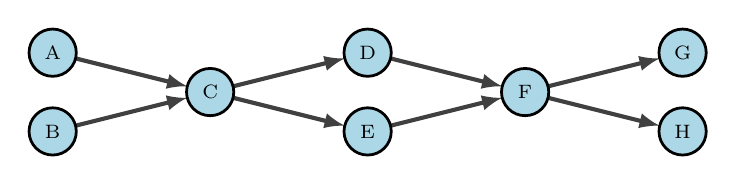
\begin{tikzpicture}
\label{def:3.3}
\Vertex[label=A]{A} 
\Vertex[label=B, y=-1]{B}
\Vertex[label=C, x=2, y=-.5]{C}
\Vertex[label=D, x=4]{D} 
\Vertex[label=E, x=4, y=-1]{E}
\Vertex[label=F, x=6, y=-.5]{F}
\Vertex[label=G, x=8]{G} 
\Vertex[label=H, x=8, y=-1]{H}
\Edge[Direct](A)(C)
\Edge[Direct](B)(C)
\Edge[Direct](C)(D)
\Edge[Direct](C)(E)
\Edge[Direct](D)(F)
\Edge[Direct](E)(F)
\Edge[Direct](F)(G)
\Edge[Direct](F)(H)
\end{tikzpicture}

After running a \hyperref[alg:dfs_dir]{DFS}-based alphabetical, topological sorting algorithm, we get the following ``pre'' and ``post'' order numbers:

\begin{center}
	\begin{tabular}{||c c c||} 
		\hline
		N & Pre & Post\\ [0.5ex] 
		\hline\hline
		A & 1 & 14 \\ 
		\hline
		B & 15 & 16\\
		\hline
		C & 2 & 13\\
		\hline
		D & 3 & 10\\
		\hline
		E & 11 & 12\\
		\hline
		F & 4 & 9\\
		\hline
		G & 5 & 6\\
		\hline
		H & 7 & 8\\ [1ex] 
		\hline
	\end{tabular}
\end{center}

The sources we find are: $A$ and $B$ vertices, and the sinks are: $G$ and $H$ vertices. We also see that the sources have the highest post-order numbers, and the sinks have the lowest post-order numbers.

\begin{property}
	\label{prop:topo_sort_sinksource}
	After topologically sorting a DAG, the source vertex is guaranteed to have the highest post-order number, and the sink is guaranteed to have the lowest post-order number. 
\end{property}

We can find a topological ordering, in a DAG, by running a $DFS$ and sort by decreasing post-order number. One such ordering would be:
$$<B, A, C, E, D, F, H,G>$$

Such sorting would take $O(|V| + |E|)$ time.

If we followed a rule that vertices should be explored alphabetically, there would be 2 possible topological orderings, depending on if we started with either source nodes $\{A, B\}$. 

Otherwise, we'd have the following choices to make during exploration:
$$<B|A, C, E|D, F, H|G>$$

which gives us $2^3 = 8$ possible orderings.

\subsection{Strongly Connected Components}
Two vertices, $v$ and $w$, are \textit{strongly connected} if $\exists v \rightsquigarrow w \land w \rightsquigarrow v$.

\begin{definition}{Strongly connected component}
	\label{def:scc}
	\\The \textit{maximal} set of strongly connected vertices. I.e., we keep greedily adding strongly connected vertices until we can add no more without breaking the definition.
\end{definition}

For the DAG below, we can extract SCC's:
$$\{A\}, \{D\}, \{B,E\}$$
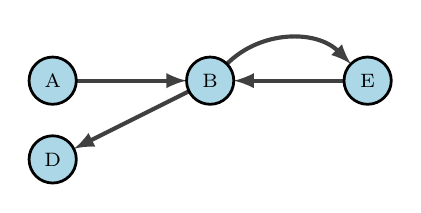
\begin{tikzpicture}
\Vertex[label=A]{A} 
\Vertex[label=B, x=2]{B}
\Vertex[label=D, y=-1]{D} 
\Vertex[label=E, x=4]{E}
\Edge[Direct](A)(B)
\Edge[Direct, bend=45](B)(E)
\Edge[Direct](E)(B)
\Edge[Direct](B)(D)
\end{tikzpicture}

An important property we can observe is \textit{every digraph is a DAG of its SCC's}:

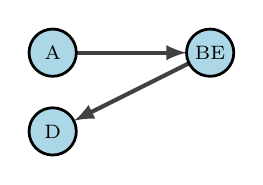
\begin{tikzpicture}
\Vertex[label=A]{A} 
\Vertex[label=BE, x=2]{B}
\Vertex[label=D, y=-1]{D} 
\Edge[Direct](A)(B)
\Edge[Direct](B)(D)
\end{tikzpicture}

Another important property is a digraph's SCC graph \textit{must be acyclic}, otherwise it would contradict the definition of an SCC, and the SCC's that are cyclic would just merge together to form a bigger SCC.\\

\textbf{Building an SCC graph from a DAG}\\
The initial step for this algorithm is crucial- we must pick a \textit{sink} node to begin with. The reason is we want to take advantage of component \textit{reach-ability}, i.e. we want our exploration step to visit only nodes in the component and terminate.

From \ref{prop:topo_sort_sinksource}, we can derive another property that we'll use in our SCC algorithm:

\begin{property}
	Let $G^R = (V, E^R)$ denoting that its edges are reversed. We have the following properties:
	\begin{itemize}
		\item A source node in $G$ is a sink node in $G^R$.
		\item A sink node in $G$ is a source node in $G^R$.
	\end{itemize}
\end{property}

\begin{algorithm}
	\caption{$SCC$: labels the SCC's in a DAG.}
	\label{alg:scc}
	\begin{algorithmic}[1]
		\REQUIRE $G=(V,E)$ is an digraph as an adjacency list.
		\STATE Construct $G^R$. 
		\STATE Run \hyperref[alg:dfs_dir]{$DFS(G^R)$}. 
		\STATE Order $V$ decreasing by post-order \#. 
		\STATE Run undirected \hyperref[alg:dfs_und]{$DFS(G)$} to label the components.
	\end{algorithmic}
Runs in $O(|V|+|E|)$.
\end{algorithm}

In \ref{alg:scc} we hand-wave a bit with the step that computes $G^R$. Here's two ways of how we might implement in linear time:

\textbf{Pseudo-code (in-place)}:\\
Modify \hyperref[alg:explore_digraph]{$Explore$}, at the end of the for-loop, to remove the edge $(v,w)$ and insert $(w, v)$ which should take $O(|V| + |E|)$ for adjacency lists.

\textbf{Pseudo-code (copy)}:\\
Initialize a new adjacency list of size $V$, runs in $O(|V|)$ time. For each neighbor $u$ of $v$ we explore, add a the reverse edge $(u, v)$ to the new adjacency list, which takes $O(|V|+|E|)$ time to traverse through all neighbors and edges in $G$.

\subsection{Minimum Spanning Tree}
\begin{definition}
	A tree is a connected, acyclic graph.
	\begin{enumerate}
		\item A tree on $n$ vertices has $n-1$ edges.
		\item In a tree, $\exists$ only one path between every pair of vertices.
		\item Any connected graph with $|E|=|V|-1$ is a tree.
	\end{enumerate}
\end{definition}

\begin{definition}
A spanning tree $F \subseteq E$, is a minimal-weight, connected component s.t.:
\begin{enumerate}
	\item $F$ is acyclic. 
	\item $F$ has $|V|-1=n-1$ edges.
\end{enumerate}
\end{definition}

\subsubsection{Problem}
Given an undirected graph $G = (V,E)$ with weight function $w(e),\: \forall e \in E$, find the spanning tree of minimal weight. 

Given some tree $T \subset E$, we want to minimize the weight sum: $$w(T) = \sum_{e \in T}w(e)$$.

\begin{algorithm}
	\caption{$Kruskals(G)$: finds the MST of $G$.}
	\label{alg:kruskals}
	\begin{algorithmic}[1]
		\REQUIRE $G=(V,E)$ is an undirected graph with weights $w(e), \: \forall e \in E$.
		\STATE Sort $E$ by increasing weights. \COMMENT{Sort using, e.g. merge-sort.}
		\STATE $X \gets \{\}$
		\FORALL {$e \in E$}
		\IF {$X \cup e$ doesn't have a cycle,}
			\STATE $X = X \cup e$
		\ENDIF
		\ENDFOR
		\RETURN $X$
	\end{algorithmic}
\end{algorithm}

Kruskal's algorithm runs in $O(|E|log(|V|))$ if using $MergeSort$, which runs in $O(|E|log(|V|))$ to sort $E$. How do we determine if $X \cup e$ doesn't contain a cycle? 

\begin{lemma}
	Let $comp(v), \: v \in (V,X)$ be a function that returns the component containing $v$. $X$ is what is returned from algorithm \ref{alg:kruskals}. Given edge $(u,v) \in (V,X)$, we know:
	$$comp(u) \neq comp(v) \implies X \cup e \text{ doesn't have a cycle.}$$
	This is possible in $O(log|V|)$ time if using the \href{https://en.wikipedia.org/wiki/Disjoint-set_data_structure}{union-find data structure}.
\end{lemma}

\subsection{Max-Flow}
\begin{definition}{Flow Networks}
\label{def:flow_networks}

A directed graph, $G = (V, E, s, t, c)$. Where $s, t$ is the source vertex $s \in V$ and sink vertex $t \in V$ and capacity function $c:E \mapsto \mathbb{N}$.
\end{definition}


\begin{definition}{Flow of an edge, $f_e$}
\label{prop:flow_edge}
	
A function, $f:E \mapsto \mathbb{N}$, representing the flow along an edge, $e \in E$ satisfying \ref{prop:capacity} and \ref{prop:conservation}.
\end{definition}

\begin{definition}{$size(f)$}
\label{prop:size}
	
Flow size represents the total flow of the network and has a useful property:
	
$$\text{Total flow out of } s = \text{Total flow into } t$$
	
given $(s, t)$ are the source and sink vertices in \ref{def:flow_networks}.
\end{definition}

\begin{definition}{Available Capacity}
\label{def:available_cap}

The available capacity at some $e \in E$ is:
$$c_e - f_e$$
\end{definition}

\begin{definition}{Saturated edge}
\label{def:sat_edge}

An edge $e \in E$ is \textit{saturated} if $f_e = c_e$.
\end{definition}

\begin{definition}{Flow-in to $v$}
\label{def:flowin}
$$\sum_{\overrightarrow{wv} \in E}{f_{wv}}$$
\end{definition}

\begin{definition}{Flow-out of $v$}
\label{def:flowout}
$$\sum_{\overrightarrow{vz} \in E}{f_{vz}}$$
\end{definition}

\begin{definition}{Feasible flow}
	
	$f$ is a a feasible flow if \ref{prop:capacity} and \ref{prop:conservation} conditions hold.
\end{definition}

\begin{definition}{$\text{Capacity constraint}$}
\label{prop:capacity}
$$\forall e \in E, \, 0 \leq f_e \leq c_e$$
\end{definition}

\begin{definition}{$\text{Conservation of flow}$}
\label{prop:conservation}

Given source and sink node $(s,t) \in E$:
$$\forall v \in V - \{s \cup t\}, \, \text{flow-in to } v = \text{flow-out of } v$$ 
\end{definition}

\begin{definition}{$\mathcal{P}$}
\label{prop:cal_p}	

	$\mathcal{P}$ is a path connecting $(s,t) \in G^f$ with some available capacity $\in f$,  see $\ref{def:available_cap}$. Remember, $G^f$ is \textit{built} based on \ref{residual_net}. I.e., $\mathcal{P}$ is an $f$-augmenting \textit{st-path} $\in G^f$
\end{definition}

\subsubsection{Problem}
The Max-Flow problem is: given a flow network, $G$, find $f$ that maximizes $size(f)$, \ref{prop:size}.

\subsubsection{Algorithm Idea}
\begin{algorithm}
\caption{$NaiveMaxFlow$}
\label{alg:naive_max_flow}
\begin{algorithmic}[1]
	\STATE Initialize flow network, $f$: $f_e = 0, \, \forall e \in E$
	\STATE Find some $\mathcal{P}$ \COMMENT{Can use $DFS$ or $BFS$ for this}
	\WHILE {$\exists \mathcal{P}$}
		\STATE $c(\mathcal{P}) \gets \min_{\forall e \in \mathcal{P}} (c_e-f_e)$
		\STATE Augment $f$ by $c(\mathcal{P})$ along $\mathcal{P}$
	\ENDWHILE
\end{algorithmic}
\end{algorithm}

\subsubsection{Residual Network, $G^f$}
\label{residual_net}
$G^f$ is useful for finding the max-flow because it lets us augment $f$ with back-edges. It is related to the original, network graph $G$:

$$G^f = (V, E^f)$$

There are constraints to be met before adding an edge $e \in E$ to $E^f$. The first is for forward edges:

\begin{definition}
\label{def:add_unsat_2_resid}
$$\overrightarrow{vw} \in E \land f_{vw} < c_{vw} \to \text{ add } \overrightarrow{vw} \text { to } E^f \text { with capacity } c_{vw} - f_{vw}$$
\end{definition}

and for back-edges:

\begin{definition}
\label{def:add_back_edge_unsat_2_resid}
$$\overrightarrow{vw} \in E \land f_{vw} > 0 \to \text{ add } \overrightarrow{wv} \text { to } E^f \text { with capacity } f_{vw}$$
\end{definition}

\begin{remark}
The reason we do not want anti-parallel edges is because if $G$ had some, we could not construct $G^f$ with forward and back-edges as noted in \ref{residual_net}.
\end{remark}

\begin{algorithm}[H]
\caption{$FordFulkerson$}
\label{alg:ford_fulk}
\begin{algorithmic}[1]
	\REQUIRE $c : E \to \mathbb{N}$ \COMMENT{This is a crucial limitation for $FordFulkerson$ to work}
	\STATE Initialize flow network, $f$: $f_e = 0, \, \forall e \in E$
	\WHILE {$\exists \mathcal{P} \in G^f$}
		\STATE Find $\mathcal{P}$
		\STATE $c(\mathcal{P}) \gets \text{the minimum capacity along } \mathcal{P}$
		\STATE Augment $f$ by $c(\mathcal{P})$ unit along $\mathcal{P}$
	\ENDWHILE
	\RETURN {$f$}
\end{algorithmic}
\end{algorithm}

In \ref{alg:ford_fulk}, we augment by increasing flow along forward edges by $c(\mathcal{P})$, and decreasing flow by $c(\mathcal{P})$ for back-edges. 

\textbf{Correctness}

The proof-of-correctness relies on the max-flow = min-cut theorem, \ref{thm:maxflowmincut}. 

\textbf{Time Complexity}

Due to the requirement in \ref{alg:ford_fulk}, the flow will increase by $\geq 1$ unit per round. How do we determine how many rounds then? Let $C=$ size of max flow. Given that the flow must increase by $\geq 1$ per round, then we know there are $\leq C$ rounds. 

It takes $O(|V|)$ time to update $G^f$, and it takes $O(|E|)$ time, assuming $|E| \geq |V|-1$ since $G$ may have multiple cycles, by running $DFS$ or $BFS$ to find $\mathcal{P}$ left in the loop. Augmenting $f$ in the loop is also $O(|V|)$, thus the running time is dominated by $O(|E|)$. 

We must take into account that there's $\leq C$ rounds we iterate through, thus the final running time is \textit{pseudo-polynomial} at:

$$O(|E|C)$$

An excellent \href{https://stackoverflow.com/questions/19649026/is-network-flow-pseudo-polynomial-time}{discussion} on what pseudo-polynomial means. \href{https://en.wikipedia.org/wiki/Ford%E2%80%93Fulkerson_algorithm#Integral_example}{Worst-case, integral example}.
	
\begin{algorithm}
	\caption{$EdmonsKarp$}
	\label{alg:edmons_karp}
	\begin{algorithmic}[1]
		\REQUIRE $c : E \to \mathbb{N}$ \COMMENT{This is a crucial limitation for $FordFulkerson$ to work}
		\STATE Initialize flow network, $f$: $f_e = 0, \, \forall e \in E$
		\WHILE {$\exists \mathcal{P} \in G^f$}
		\STATE Find $\mathcal{P}$
		\STATE $c(\mathcal{P}) \gets \text{the minimum capacity along } \mathcal{P}$
		\STATE Augment $f$ by $c(\mathcal{P})$ unit along $\mathcal{P}$
		\ENDWHILE
		\RETURN {$f$}
	\end{algorithmic}
	\href{https://classroom.udacity.com/courses/ud401/lessons/8e8db62c-39bd-4dc2-bbe7-b9774e41756f/concepts/77dcde9a-43f0-4eea-889b-14b1ec034a28}{TODO}.
\end{algorithm}

\subsection{Max-flow = Min-cut}
\begin{lemma}
\label{lem:aug_path}
For a flow, $f^*$: $$\mathcal{P} \notin G^{f^*} \implies f^* \text{is a max-flow}$$
	
Where $\mathcal{P}$ is \ref{prop:cal_p}.
\end{lemma}

\begin{definition}{\textit{st-cut} and its capacity}
\label{def:st_cut_cap}

An \textit{st-cut} is a partition of $V = L \cup R$, s.t. $s \in L, t \in R, L \cap R = \emptyset$. The capacity from $L$ to $R$ is calculated as:

$$c(L,R) = \sum_{\overrightarrow{vw} \in E : v \in L, w \in R} c_{vw}$$
\end{definition}

\begin{claim}
\label{clm:in_out_flow}
For any flow $f$ and any st-cut $(L,R)$:
$$size(f) = f^{out} (L) - f^{in} (L)$$
\end{claim}

\begin{proof}
	\begin{flalign*}
		f^{out}(L) - f^{in}(L) &= \\
		\shortintertext{First term captures flow \textit{out} of $L$, second term captures flow \textit{into} $L$.}
		&= \sum_{\overrightarrow{vw} \in E:v \in L, w \in R}f_{vw} - \sum_{\overrightarrow{wv} \in E:w \in R, v \in L}f_{wv}\\ 
		\shortintertext{We add and subtract a third and fourth term, representing representing the sum of flows \textit{within} $L$.}
		&+ \sum_{\overrightarrow{vw} \in E:v \in L, w \in L}f_{vw} - \sum_{\overrightarrow{wv} \in E:w \in L, v \in L}f_{wv}\\ 
		\shortintertext{The first and third terms above consider edges from $v \in L$ to $R$, plus edges within $L$. Combined together, we have \textit{all edges} out of $v \in L$, represented as the first term below. Similarly, the second and last terms give the total flow \textit{into} $v \in L$.}
		&= \sum_{v \in L} f^{out}(v) - \sum_{v \in L} f^{in}(v)\\ 
		\shortintertext{We tease out vertex $s$ from the two flow summations above and add $f^{out}(s)$ to maintain equivalence. There is no $f^{in}(s)$ term below, because \emph{$s$ never has flow into it.}}
		&= \sum_{v \in L-s}(f^{out}(v) - f^{in}(v)) + f^{out}(s)\\
		\shortintertext{By conservation of flow, \ref{prop:conservation}, the flow summations in and out of $v$ cancel out.}
		&= \sum_{v \in L-s}0 + f^{out}(s)\\
		\shortintertext{By \ref{prop:size}.}
		&= f^{out}(s) = size(f)&
	\end{flalign*}
\end{proof}

\begin{claim}
\label{clm:size_f_star_is_clr}
	For some $f^*$ generated from $FordFulkerson$:
	$$size(f^*) = c(L,R)$$	
\end{claim}

\begin{proof}
Let $f^*$ be a flow without a path $\mathcal{P} \in G^{f^*}$. We now perform an st-cut, $(L, R)$ by definition \ref{def:st_cut_cap}.

Since $f^*$ has no $\mathcal{P} \in G^{f^*}$, we know that sink $t$ \textbf{can't} be reachable from source $s$ in $G^{f^*}$ by \ref{prop:cal_p}. 

We let $L$ be the set of reachable vertices from $s \in G^{f^*}$, and $R = V - L$. From this, we know $s$ must be in $L$ since $s$ can reach itself, and $t$ must be in $R$, since it contains the set of vertices \textit{unreachable} from $s$. 

It follows that $t \notin L$, because if so, $\exists s \rightsquigarrow t$, which contradicts that $f^*$ has no $\mathcal{P} \in G^{f^*}$.

Taking an st-cut $(L,R)$, we derive a few facts:

\begin{enumerate}
	\item $\forall \overrightarrow{vw} \in E : v \in L, w \in R$, $\overrightarrow{vw}$ is a saturated edge. Otherwise, $\overrightarrow{vw} \in G^{f^*}$ by \ref{def:add_unsat_2_resid}, contradicting $\mathcal{P} \notin G^{f^*}$ because $G^{f^*} \cup \overrightarrow{vw} \implies \exists s \rightsquigarrow t$.
	\item Total $f^{out}(L) = c(L,R)$ by \ref{def:available_cap}.
	\item  $\forall \overrightarrow{wv} \in E : w \in R, v \in L$, $f_{wv} = 0$, otherwise its back edge, $\overrightarrow{vw} \in G^{f^*}$ by \ref{def:add_back_edge_unsat_2_resid}, contradicting $\mathcal{P} \notin G^{f^*}$.
	\item Thus, total $f^{in}(L) = 0$.
\end{enumerate}

Now we may conclude \ref{clm:size_f_star_is_clr} from such facts:
\begin{align*}
size(f^*) &=\\
\shortintertext{From claim \ref{clm:in_out_flow},}
f^{out}(L) - f^{in}(L)&=\\
c(L,R)- 0&=\\
c(L,R)
\end{align*}
\end{proof}

\begin{theorem}{Max-flow = Min-cut}
\label{thm:maxflowmincut}

I.e., the size of max-flow = the minimum capacity of some \textit{st-cut}.
\end{theorem}

To prove \ref{thm:maxflowmincut}, we first prove $\text{max-flow} \leq \text{minimum st-cut}$, then we prove the reverse inequality, $\text{max-flow} \geq \text{minimum st-cut}$.

\begin{proof}
	To prove that $$\text{max-flow} \leq \text{minimum st-cut},$$ we can prove an easier, more general property: for any flow $f$ and any st-cut $(L,R)$:
	
	$$size(f) \leq c(L,R) \implies \text{max-flow} \leq \text{minimum st-cut}$$
	
	where, $c(L,R)$ is the capacity defined in \ref{def:st_cut_cap}. The intuition being that the max-flow of $size(f)$ is just a special case of some $size(f)$, and that the minimum $c(L,R)$ is just a special case of finding some $c(L,R)$.
	
	\begin{align*}
		\shortintertext{By claim \ref{clm:in_out_flow}, we know:}
		size(f) = f^{out} (L) - f^{in} (L)\\
		\shortintertext{It's trivial that $f^{in}(L)$ subtracted from $f^{out}(L)$ makes $f^{out}(L)$ smaller:}
		f^{out} (L) - f^{in} (L) \leq f^{out}(L)\\
		\shortintertext{Along every edge $e$ leaving $L$, we know $f_e$ is $\leq c_e$ by \ref{prop:capacity}:} 
		f^{out} (L) - f^{in} (L) \leq f^{out}(L) \leq c(L,R)
	\end{align*}
	Thus the total flow out of $L$ is at most the total capacity of the edges from $L$ to $R$:

	$$f^{out}(L) \leq c(L,R)$$

	We now show the reverse inequality:
	$$\text{max-flow} \geq \text{minimum st-cut}$$
	Rephrased as:
	$$\text{after maximizing over $f$, } size(f) \geq \text{minimal }c(L,R)$$
	To do so, take some $f^*$ produced from the $FordFulkerson$ algorithm. From \ref{lem:aug_path}, we know that $f^*$ is a max-flow. We want to construct an $(L,R)$ from $f^*$ s.t.:
	$$size(f^*) = c(L,R)$$
	How does the above equality imply $\text{max-flow} \geq \text{minimum st-cut}$? Because we know the max $size(f)$ is at least the $size(f^*)$- note that $f^*$ is just \textit{some} flow calculated during the execution of $FordFulkerson$. 
	So, if we maximize over flow $f$:
	$$size(f) \geq size(f^*) = c(L,R)$$
	Now, how does $c(L,R)$ compare to $\text{minimal }c(L,R)$? Obviously, $c(L,R) \geq \text{minimal }c(L,R)$.
	Using the hypothesis above, we now just need to prove the middle equality term of:
	$$\text{maximum } size(f) \geq size(f^*) = c(L,R) \geq \text{minimal }c(L,R)$$
	which we've proved in \ref{clm:in_out_flow}.
\end{proof}

\section{Reductions}
In this section we discuss methods to reduce problems to a form that can be solved by a black-box algorithm such as max-flow.

\subsection{Generalization (Circulation and Demand)}
There's a large class of problems that could be solved with max-flow, but require a bit of massaging. This class of problems are usually reduced to the following, before being finally reduced to max-flow:

\begin{enumerate}
	\item Circulation with Demands (C\&D)
	\item C\&D with lower bounds
\end{enumerate}

\begin{definition}{Demand, $d_v$}
\label{def:demand}
	\\A node, $v \in V$ can be associated with a demand, $d_v$. 
	\\$d_v >0$ indicates $v$ demands $d_v$ units. 
	\\$d_v < 0$ indicates $v$ has a \textit{supply} of $-d_v$ units.
\end{definition}

\begin{definition}{Feasible circulations}
	\label{def:feas_circulation}
	\\Given demands $\{d_v\}$, a \textit{feasible} circulation is function $f: E \mapsto \mathbb{R}^+$ that satisfies:
	
	\begin{enumerate}
		\item (Capacity condition) $\forall e \in E, 0 \leq f(e) \leq c(e)$
		\item (Demand condition) $\forall v \in V, f^{in}(v) - f^{out}(v) = d_v$
	\end{enumerate}

	I.e., total supply must equal total demand:
	$$\exists \text{ a feasible circulation with demands } \{d_v\} \implies \sum_{v \in V}{d_v} = 0$$
\end{definition}

\begin{corollary}{$D$}
	\\It follows from \ref{def:feas_circulation} that:
	$$D = \sum_{v \in V: d_v > 0}{d_v} = \sum_{v \in V: d_v < 0}{-d_v} = \sum_{v \in V}{d^{in}(v)} =\sum_{v \in V}{d^{out}(v)}$$
\end{corollary}

\say{We can reduce the problem of finding a feasible circulation with demands $\{d_v\}$ to the problem of finding the max st-flow in a different network.}

To do so, we first need to convert our $G$ graph to the familiar flow network, \hyperref[def:flow_networks]{$G' = (V, E, s,t, \{c_e\})$}.
Let $S$ be the set of ``flow-generating'' sources, and $T$ be the set of ``flow-absorbing'' sinks:

\begin{enumerate}
	\item $\forall v \in S$, attach a ``super-source'', $(s^*,v)$, with $c_e = -d_v$.
	\item $\forall v \in T$, attach a ``super-sink'', $(v,t^*)$, with $c_e = d_v$.
\end{enumerate}

We carry over everything else from $G$ to $G'$ and thus completes our structural conversion to a flow network. 

Now, \textbf{where did the actual reduction happen} as we transformed $G \to G'$? Adding $s^*$ to ``supply'' the extra flow to the sources, and $t^*$ to ``siphon'' the extra flow out of the sinks is the reduction. Now we seek the max $s^*t^*$ flow $\in G'$. 

What is the upper bound of any $s^*t^*$ flow? It must be $D$ due to how we set what the capacities during the reduction phase, and if we take any cut $(A,B)$ with $A = \{s^*\}$ we see that $c(A,B) = D$ by \hyperref[thm:maxflowmincut]{max-flow min-cut theorem}.

The reduction can be concluded and proven equivalent to the max-flow problem with the following lemmas:

\begin{lemma}
	$\exists$ a feasible circulation with demands $\{d_v\} \in G \iff$ the max $s^*t^*$ flow $\in G' = D$. 
\end{lemma}

\begin{lemma}
	The graph $G$ has a feasible circulation with demands $\{d_v\} \iff \forall c(A,B), \sum_{v \in B}{d_v \leq c(A,B)}$. \textbf{Note} that such cut need not be an \hyperref[def:st_cut_cap]{st-cut} in this context.
\end{lemma}

Now we generalize even further by adding \textit{lower bounds}. 

\begin{definition}{Lower bound capacities}
	\label{def:low_bounds}	
		\begin{enumerate}
			\item (Capacity condition) $\forall e \in E, l(e) \leq f(e) \leq c(e)$
			\item (Demand condition) $\forall v \in V, f^{in}(v) - f^{out}(v) = d_v$
		\end{enumerate}
\end{definition}

As before, we need to again verify what a feasible circulation under these new rules.

\textbf{TODO}: Finish the lower bound K\&T chapter and reconcile with \href{https://classroom.udacity.com/courses/ud401/lessons/98e96502-88a9-4c08-9737-5bfce78d6248/concepts/12561c77-2bcd-45e0-aae5-e7c4d57eb2ef}{lectures}.

\subsection{Perfect Bipartite matching}
\begin{definition}{Bipartite graphs}
	\label{def:bipartite_graphs}
	\\In general a bipartite graph $G=(V_1 \cup V_2, E)$ s.t. each edge has one endpoint in $V_1$ and the other in $V_2$.
\end{definition}

An example of this problem is \textit{matchmaking} for couples. Let $G(V,E)$ be an un-directed graph with vertices that are either male ($M \subset V$) or female ($F \subset V$). An edge, $e \in E$ denotes a match between two people, $v \in V$. Is it possible to choose couples s.t. everyone has \textit{exactly one partner}, i.e. a perfect match?

We first need to translate $G$ into the flow-network: $$G'(V,E',s,t,c: E' \mapsto \mathbb{N})$$

Assume $G$ is bipartite and $|M|=|F|$, i.e. even \# of males and females s.t. couples could be formed.

We add a source $s$ node and connect it to all $v \in M$. We then connect all $v \in F$ to a sink node, $t$. This fulfills the $s,t$ node requirement for $G'$.

Then, we set the max-capacity to all $e \in E'$ to 1, i.e. our capacity function is now $c : E' \mapsto 1$.

Now we run $FordFulkerson$, \ref{alg:ford_fulk}, on $G'$ to generate $f^*$. If $|f^*| = $ the total number of possible couples, we have achieved a perfect match.

\textbf{Intuition}: maxing out the capacity to 1 gives us a nice property which allows us to completely saturate some $\mathcal{P}$ in any given iteration of \ref{alg:ford_fulk}. 

Recall from \ref{def:add_back_edge_unsat_2_resid} that only back-edges are added for saturated edges in $G'$, and once we augment along $\mathcal{P}$ in some step, the next build of ${G'}^{f^*}$ will have all back-edges of edges that comprised of $\mathcal{P}$ pre-augmentation. 

Since $G$ is well-formed, from a couples and bipartite perspective, we know that if some $\mathcal{P}$ was augmented, at least one male and female along $\mathcal{P}$ were saturated. By \ref{prop:conservation}, we know the remaining edges along $\mathcal{P}$ are also saturated. 

Thus no other $\mathcal{P'}$, such as a $\mathcal{P}$-overlapping one, can send any more flow across $\mathcal{P}$, otherwise a vertex could receive more flow from more than one vertex (analogous to a person matching with more than one person), which breaks our definition of a couple-matching.

\subsection{Direct Bipartite matching}
\begin{algorithm}
	\caption{$BFS$}
	\label{alg:bfs}
	\begin{algorithmic}[1]
		\REQUIRE $Q$ is a queue, rooted graph $G$, root vertex $v$,\\discovered array $disc : V \mapsto \{0, 1\}$.
		\STATE $disc[v] \gets 1$
		\STATE $Q$.enqueue($v$)
		\WHILE {$Q$ isn't empty}
			\STATE $n \gets$ $Q$.dequeue()
			\IF {$n$ is some goal}
				\RETURN $n$
			\ENDIF
			\FOR {all neighbors $u$ of $n$}
				\IF {$\neg disc[u]$}
					\STATE $disc[u] \gets 1$
					\STATE $parent[u] \gets v$
					\STATE $Q$.enqueue($u$)
				\ENDIF
			\ENDFOR
		\ENDWHILE
		\RETURN $parent[*]$
	\end{algorithmic}
Runs in $O(|V|+|E|)$.
\end{algorithm}

\begin{definition}{Matching edges}
\label{def:match_edge}
	\\A \textit{matching}, $M \in G$ is a set of edges with:
	\begin{enumerate}
		\item Pairwise, non-adjacent edges.
		\item Acyclic.
		\item No two edges share a common vertex.
	\end{enumerate}
\end{definition}

\begin{definition}{Covered vertex}
	\label{def:covered_vtx}
	\\A vertex is \textit{covered} by $M$ if it is an endpoint of any $e \in M$.
\end{definition}

\begin{definition}{Alternating path}
	\label{def:alt_path}
	\\A path, $a := u \rightsquigarrow v$, s.t.:
	\begin{enumerate}
		\item $|a|$ is odd.
		\item $u, v$ are non-covered vertices.
		\item $a$'s edges alternate between $M$ and $E-M$.
	\end{enumerate}
\end{definition}

\begin{definition} {Maximal matching of $M$}
	\label{def:maximal_m}
	\\$M$ is \textit{maximal} if $\nexists e \in E \land e \notin M$ that can be added to $M$ because it would cause $M$ to \textbf{no longer be a matching graph}. \href{https://brilliant.org/wiki/matching/}{Reference}.
	
	A maximal matching is only local (greedy), i.e. it does not mean you found the \textit{best matching overall}- that is the \textbf{maximum} matching. \href{https://piazza.com/class/k52uzg6xjkl5xz?cid=618_f4}{Reference}.
\end{definition}

\begin{claim}
	$M$ is maximal $\iff \nexists$ an alternating path w.r.t. it.
\end{claim}

\begin{proof}	
	A \textit{minimum} alternating path encloses 1 matching edge. There is another matching we could do that increases the maximal matching, i.e. making the two end-edges matching with a total of 2 matches.
	
	A corollary is our original alternating path is no longer an alternating path since they no longer begin and end with covered vertices.
	
	Thus, it is a contradiction to have a maximal $M$ in an alternating path.
	
	\textbf{TODO:} The proof above only covers the base case so it's not a general enough proof. We also need to prove the other direction, \href{http://www-cs-students.stanford.edu/~csilvers/proof/node4.html}{see this reference}.
\end{proof}

\begin{claim}
	Given a bipartite graph, $G = (V_1 \cup V_2, E)$, $\exists$ an algorithm to find some \hyperref[def:alt_path]{alternating path} $\in G$ in $O(|V|+|E|)$ using a modified $BFS$ algorithm.
\end{claim}

\textbf{HINT:} use properties of:
\begin{enumerate}
	\item DAGs
	\item BFS traversal
	\item Bipartite graphs
	\item Alternating paths
	\item Match edges
\end{enumerate}
to construct a solution.

\begin{proof}
	 Let $A \subseteq V_1$ and $B \subseteq V_2$  be the set of uncovered edges.
	
	A post-condition we can derive is- if an alternating path is found, we know it crossed $V_1, V_2$ at least three times:
	\begin{enumerate}
		\item Starting at an uncovered vertex, $u \in A$, it crosses $V_1, V_2$ along an unmatched edge to some covered vertex, $v \in V_2 - B$.
		\item From $v$, it crosses some matched edge, $e \in M$ back to some covered vertex in $V_1-A$.
		\item To maintain an alternating path, there must exist an uncovered vertex, $v' \in B$ to cross over to next.
	\end{enumerate}
	
	It's preferred to encode such invariants, and pre/ post-conditions into $BFS$, whether data-structurally or algorithmically. This makes the proof of correctness easier since modifications to the core algorithm are minimized. We know from \hyperref[alg:bfs]{$BFS$} that during traversal it checks if the current vertex meets some terminating condition.
	
	To minimally change $BFS$, we can encode our post-condition by making the terminating condition be: $n \in B \to$ terminate. This is incomplete, because an uncovered vertex $\in A$ can be adjacent to yet another uncovered vertex $\in B$, i.e. an unmatched edge ($e \notin M$) can be traversed first. The suggested model seems to leave this out. 
	
	We can overcome this with a technical detail, by extending our terminating condition to also ensure that $parent[v] \neq r$, where $r$ is the root vertex we begin at. 
	
	During traversals, we now must decide which edge to take. For instance, say we are traversing $r$'s neighbor $n \in B$, and $n$ is incident on both a matched and unmatched edge. Since we're looking for alternate paths, $n$ should never take the unmatched edge, otherwise it would not be alternating.
	
	We can encode this property by transforming $G$ to $\overrightarrow{G}$, s.t. edges are directed from $V_1$ to $V_2$ if they're \textbf{$\notin$} $M$, otherwise the edge directions will be reversed. Now, paths that lead to alternate paths are analogous to valid, directed traversals. It is left to prove that constructing $\overrightarrow{G}$ is bounded by $O(|V|+|E|)$, otherwise the claim is proven given we run $BFS$ on some start vertex $r \in A$.
\end{proof}

\begin{claim}
	Given a bipartite graph, $G = (V_1 \cup V_2, E)$, $\exists$ an algorithm to find a \hyperref[def:maximal_m]{maximal matching} $M \in G$ in $O(|V||E|)$.
\end{claim}

\begin{proof}
	\textbf{Intuition}: We only need to find a maximal matching, so we can use a greedy algorithm that grows $M$ by adding valid matches until $\nexists e \in E-M$ s.t. adding $e$ to $M$ \hyperref[def:match_edge]{invalidates} it.
	
	We can loop through each $v \in V$, and add the first of $v$'s edges that have not already been matched to $M$. It's left to prove this meets $O(|V||E|)$, however the correctness is supported \href{https://www.cs.dartmouth.edu/~ac/Teach/CS105-Winter05/Notes/kavathekar-scribe.pdf}{here}.
\end{proof}

\begin{claim}
	Given a bipartite graph, $G = (V_1 \cup V_2, E)$, $\exists$ an algorithm to find a \hyperref[def:maximum_m]{maximum matching} $M \in G$ in $O(|V||E|)$.
\end{claim}

\begin{proof}
	\textbf{TODO}. Also, check follow-ups \href{https://piazza.com/class/k52uzg6xjkl5xz?cid=705}{here} if any.
\end{proof}

\subsection{Hall's theorem}
Given a bipartite graph, $G = (V_1 \cup V_2, E)$, where $V_1$ are boys, $V_2$ are girls, and $|V_1|=|V_2|$:
$$\exists \text{ a perfect matching} \iff \text{any subset } S \subseteq V_1 \text{ connects to at least } |S| \text{ girls.}$$
\href{https://www2.cs.duke.edu/courses/spring19/compsci230/Notes/lecture14.pdf}{Reference.}

\begin{proof} 
\textbf{TODO}:
($\Rightarrow$): In this direction, we need to encode what a \textit{perfect matching} is as a neighborhood function. Use \href{http://www-cs-students.stanford.edu/~csilvers/proof/node4.html}{directional proofs} as a guidance.
\\($\Leftarrow$): Reduce to a flow-network and use \hyperref[thm:maxflowmincut]{max-flow min-cut} theorem to prove in the other direction.
\end{proof}

\subsection{Image segmentation}
\textbf{TODO.}

\section{Computational Complexity}
\subsection{Reducing Optimization to Search (or vice-versa)}
\begin{algorithm}
	\caption{\textit{TSP}, traveling salesman (search) problem}
	\label{alg:tsp_bb}
	\hspace*{\algorithmicindent} \textbf{Input:} A distance matrix and budget $b$.\\
	\hspace*{\algorithmicindent} \textbf{Output:} A tour passing through all cities and has length $\leq b$, if there exists one.
\end{algorithm}
\begin{algorithm}
	\caption{\textit{TSP-OPT}, traveling salesman (optimization) problem}
	\label{alg:tspopt}
	\hspace*{\algorithmicindent} \textbf{Input:} A distance matrix.\\
	\hspace*{\algorithmicindent} \textbf{Output:} The shortest tour passing through all cities.
\end{algorithm}

If \ref{alg:tsp_bb} $\in P$, can \ref{alg:tspopt} be shown to also be $\in P$? Yes:

\begin{proof}
	We assume \ref{alg:tsp_bb} outputs \textit{false} if no such tour is found, and the idea is to use it as a sub-routine in \ref{alg:tspopt}.\\
	Note that the signature for \ref{alg:tspopt} does not have a budget as input, but \ref{alg:tsp_bb} does. This is a hint for the solution.\\
	\ref{alg:tspopt} cares about the \textit{optimum} shortest tour only. Since \ref{alg:tsp_bb} outputs a tour of length $\leq b$ or false, we can repeatedly call it to find the optimum.
	We calculate $c$, the optimum cost (distances), by iterating through all edges in $E$ and summing their distances together.\\
	Now we can modify $BinarySearch$ s.t. it calls \ref{alg:tsp_bb} on $c$, $(0, \lfloor c/2 \rfloor)$, and $(\lfloor c/2 \rfloor +1, c)$. The reasoning being that if \ref{alg:tsp_bb} doesn't return false when searching on the former interval, we know the optimum shortest tour exists within that range, and vice-versa for the latter. \href{https://cseweb.ucsd.edu/classes/sp08/cse101/hw/hw6soln.pdf}{Reference}.
\end{proof}

\subsection{Search versus Decision}
\begin{algorithm}[H]
	\caption{\textit{Rudrata-Path-D}, Rudrata st-path (decision)}
	\label{alg:rudrata_d}
	\hspace*{\algorithmicindent} \textbf{Input:} A rooted graph $G$.\\
	\hspace*{\algorithmicindent} \textbf{Output:} True if a Rudrata st-path is found, false otherwise.
\end{algorithm}
\begin{algorithm}
	\caption{\textit{Rudrata-Path-S}, Rudrata st-path (search)}
	\label{alg:rudrata_s}
	\hspace*{\algorithmicindent} \textbf{Input:} A rooted graph $G$.\\
	\hspace*{\algorithmicindent} \textbf{Output:} The Rudrata st-path, if there exists one.
\end{algorithm}

If we are given a polynomial algorithm that solves \ref{alg:rudrata_d}, can we use it to build a polynomial algorithm that solves \ref{alg:rudrata_s}? Yep:

\begin{proof}
	Run a modified \hyperref[alg:bfs]{$BFS$} starting at root $s$. At each level, we run \ref{alg:rudrata_d} on each neighbor. If it returns true, we queue up its neighbors. If false, we do not queue its neighbors.
	
	Upon termination, the output will be the result of $BFS$ (paths via parent links from $t$ back to $s$), or an empty tree signifying that there is no Rudrata st-path.\\
	
	The \href{https://cseweb.ucsd.edu/classes/sp08/cse101/hw/hw6soln.pdf}{reference solution} runs \ref{alg:rudrata_d} on $G - \{e\}$ for some $e \in E$ in a loop. If true, we know a Rudrata st-path can be found on another path, so $e$ is permanently removed from $G$. Otherwise, the Rudrata st-path is along $e$, so it cannot be removed. Loop until nothing is left but the Rudrata st-path.
\end{proof}

\end{document}
